\documentclass[11pt]{article}

\usepackage[margin=1in]{geometry}
\usepackage[T1]{fontenc}
\usepackage[utf8]{inputenc}
\usepackage{csquotes}
\usepackage{longtable}


\usepackage[backend=biber,style=numeric,sorting=none,maxnames=3,minnames=1]{biblatex}
\addbibresource{bib/refs.bib}
\addbibresource{../bib/common.bib}

\usepackage{hyperref}

\usepackage{bucket}

\hypersetup{
  colorlinks = true,
  linkcolor  = bucketblue,
  citecolor  = bucketblue,
  urlcolor   = bucketblue,
}

\newcommand{\emp}[1]{\textcolor{bucketgray}{\footnotesize [empirical: #1]}}
\newcommand{\bm}[1]{\textcolor{bucketgray}{\footnotesize [bm:#1]}}
\newcommand{\cmd}{\texttt{npx ts-node scripts/build-solvability-frontier-report.ts}}
\newcommand{\bt}{\emp{output/solvability-frontier/report/backtest.json, 2026-10-06, \cmd}}
\newcommand{\fr}{\emp{output/solvability-frontier/report/frontier.json, 2026-10-06, \cmd}}
\newcommand{\pr}{\emp{output/solvability-frontier/report/predictions.json, 2026-10-06, \cmd}}
\newcommand{\mk}{\emp{output/solvability-frontier/report/makeup/makeup.json, 2026-10-06, python3 tools/solvability-atlas/makeup.py --publish}}

\glossentry{reach}{reach}%
  {https://github.com/gianyrox/bucket-foundation/blob/dev/src/lib/research-os/solvability-frontier.ts}%
  {A problem's highest cosine similarity to a solved problem other than itself, over its stored neighbours; see \Cref{def:reach}.}
\glossentry{frontier}{frontier}%
  {https://github.com/gianyrox/bucket-foundation/blob/dev/src/lib/research-os/solvability-frontier.ts}%
  {The reach value at the 10th percentile of solved problems' reach; a problem at or above it is inside, below it outside; see \Cref{def:frontier}.}
\glossentry{growth}{growth}%
  {https://github.com/gianyrox/bucket-foundation/blob/dev/src/lib/research-os/solvability-frontier.ts}%
  {For a problem beyond the frontier, one plus the number of beyond problems among its stored neighbours that sit at or above the threshold from it; see \Cref{def:growth}.}
\glossentry{reachclass}{reach class}%
  {https://github.com/gianyrox/bucket-foundation/blob/dev/src/lib/research-os/solvability-predictions.ts}%
  {One of four labels for an open problem: close to known results, borderline, needs a new idea, unsampled; see \Cref{def:class}.}
\glossentry{backtest}{backtest}%
  {https://github.com/gianyrox/bucket-foundation/blob/dev/src/lib/research-os/solvability-backtest.ts}%
  {The frontier rule applied at a past cutoff year to the problems posed by then, scored against their 2026 status; see \Cref{def:backtest}.}

\title{The Solvability Frontier: Which Open Problems Sit Next to Solved Ones, and a Backtest of the Rule}
\author{Bucket Foundation}
\date{2026-10-06}

\begin{document}
\maketitle

\begin{abstract}
We embed 5,080 problem statements across seven canon branches with a small sentence encoder, call a problem's \term{reach}{reach} its highest similarity to a solved problem, and draw a \term{frontier}{frontier} at the 10th percentile of solved problems' reach, 0.781 on this set \fr. Open problems are sorted into a \term{reachclass}{reach class}: 251 close to known results, 764 borderline, 911 that need a new idea and 103 in a branch with too few solved rows to judge \pr. A \term{backtest}{backtest} at cutoffs 2005 and 2021 scores the rule on the questions posed by those years under two outcome codings. Settled only (solved in 2026): at 2005 the inside rows settle at 21\% against 6\% outside (112 and 71 rows, ratio 3.804, permutation $p=0.006$, AUC 0.800), at 2021 at 12\% against 1\% (238 and 126 rows, ratio 14.824, $p=0.000$, AUC 0.883) \bt; removing the solved rows that carry no resolved year, 11 and 21, drops the gaps to 13\% against 6\% ($p=0.131$) and 3\% against 1\% ($p=0.269$) \bt. Settled or advanced (solved or partial): at 2005, 46\% inside against 61\% outside (ratio 0.752, $p=0.051$, AUC 0.479), at 2021, 43\% against 39\% (ratio 1.102, $p=0.503$, AUC 0.523) \bt. The conclusion depends on how partial is coded, and partial is the uncertain column: the ingest assigned it in 2026 from a status page with no rule for how much progress counts. The embeddings and the 50 stored neighbours come from the 2026 corpus, so the test is a check against known outcomes under that leak; a forecast would need embeddings fitted on pre-cutoff text and a neighbour set frozen per cutoff.
\end{abstract}

\section{Introduction}
\label{sec:intro}

Bucket's solvability atlas lists open and closed problems with their statements, branch, status and, where known, the years they were posed and resolved. The question behind the frontier is whether an open problem that sits close in meaning to solved problems is closer to being solved, and whether an AI system working from known results could reach it. The frontier drawing answers the first clause by a rule; this paper tests the rule on problems whose outcome is known and publishes the ranked predictions for the open ones, with every number tagged to the file and command that reproduces it.

\section{Related work}
\label{sec:related}

The atlas draws on the 2005 Science list of 125 questions \autocite{kennedy2005whatdontweknow,science2005somuchmore}, the 2021 Science and Shanghai Jiao Tong University list\footnote{\url{https://www.science.org/content/resource/125-questions-exploration-and-discovery}, read from a Wayback copy of the booklet; no DOI.}, the google-deepmind formal-conjectures repository\footnote{\url{https://github.com/google-deepmind/formal-conjectures}, Apache-2.0; no DOI.} and the Wikipedia lists of unsolved problems\footnote{\url{https://en.wikipedia.org/wiki/Lists_of_unsolved_problems}, CC BY-SA 4.0; no DOI.}. The encoder is bge-small-en-v1.5, whose model card points at the C-Pack paper \autocite{xiao2023cpack}. Systems that generate and test scientific hypotheses end to end \autocite{gottweis2025coscientist,lu2024aiscientist} are the setting in which a reach score would be used; this paper measures only whether the score tracks outcomes.

\section{Preliminaries}
\label{sec:prelim}

\begin{definition}[Set]
\label{def:set}
The set is the 71 atlas problems and the 5,009 rows of \texttt{problems-sourced.tsv}, 5,080 rows once Lean theorems are left off \fr. A top-level row is solved when its status is solved. A variant is solved only when it and its parent are both solved. Each row's statement is embedded with bge-small-en-v1.5 at revision 5c38ec7, and its 50 most similar rows are stored with cosine similarity to three decimals \fr.
\end{definition}

\begin{definition}[Reach]
\label{def:reach}
The \term{reach}{reach} of a row is its highest similarity to a solved row other than itself, taken over its stored neighbours and its stored nearest solved row.
\end{definition}

\begin{definition}[Frontier]
\label{def:frontier}
The \term{frontier}{frontier} threshold $\tau$ is the 10th percentile of reach over the solved rows. A row with reach at or above $\tau$ is inside; below it, outside. An open row whose branch holds fewer than 10 solved rows is unsampled and counted outside.
\end{definition}

\begin{definition}[Growth]
\label{def:growth}
For a top-level row beyond the frontier, \term{growth}{growth} is one plus the number of beyond top-level rows among its 50 stored neighbours whose similarity to it is at or above $\tau$: the number of rows that would move inside if it were solved. Variants neither pull nor count as pulled.
\end{definition}

\begin{definition}[Reach class]
\label{def:class}
Let $u$ be the 75th percentile of reach among open rows inside the frontier. An open top-level row is \enquote{close to known results} when inside with reach at or above $u$, \enquote{borderline} when inside below $u$, \enquote{needs a new idea} when beyond, and \enquote{unsampled} when its branch holds fewer than 10 solved rows. Within a class, rows rank by growth, then reach, then id; a ranking by score with unique ids has one ordering \bm{BucketMath.Ranking.rank\_ordered}.
\end{definition}

\begin{definition}[Backtest]
\label{def:backtest}
For a cutoff year $c$, the solved set $S_c$ holds every row solved under \Cref{def:set} with a resolved year at or before $c$. The tested set holds every row posed at or before $c$ and outside $S_c$. Reach is computed as in \Cref{def:reach} against $S_c$ alone. When none of a row's stored neighbours is in $S_c$, its reach is unknown and bounded above by its 50th neighbour's similarity. The threshold $\tau_c$ is the 10th percentile of reach over the rows of $S_c$ that have a neighbour in $S_c$; the rest are counted and dropped. A tested row is inside when its reach is at or above $\tau_c$, outside when its reach or its bound is below $\tau_c$, and undecided otherwise; undecided rows are counted and left out of the rates. The outcome is the row's 2026 status under two codings reported side by side: \enquote{settled} counts solved only, \enquote{settled or advanced} counts solved or partial. A solved row with no resolved year that was posed by the cutoff is tested and scored as resolved; every table repeats its first row with those rows removed. Undecided rows are also scored under two extremes, all inside and all outside, as bounds without a $p$-value.
\end{definition}

\section{Method}
\label{sec:method}

\paragraph{Statistics.}
Per cutoff and per stratum we report the inside and outside counts, the resolved rate on each side, their ratio (inside over outside, undefined when the outside rate is zero \bm{BucketMath.Marketing.ratio}) and a two-sided permutation $p$-value: the outcomes are shuffled 10,000 times under seed 20261006 and $p$ is the share of shuffles whose absolute rate difference is at least the observed one, with one added to numerator and denominator \bt. The $p$-value so defined is positive and at most one (\Cref{app:lean}). A stratum with fewer than 10 rows on either side reports counts only. The AUC is the Mann-Whitney probability that a resolved row's reach exceeds an unresolved row's, ties counting one half.

\paragraph{Strata.}
Rows are stratified by the word count of the embedded text, under 20, 20 to 40 and over 40 words, and by branch. The bands partition the naturals (\Cref{app:lean}). The length bands exist because the dated lists are short paraphrases: their statements average 19 words against 34 for the rest of the file \bt.

\paragraph{Reproduction.}
\texttt{tools/solvability-atlas/build.sh} rebuilds the embeddings and the neighbour file; \cmd{} writes \texttt{frontier.json}, \texttt{backtest.json}, \texttt{predictions.json} and \texttt{predictions.csv} under \texttt{output/solvability-frontier/report/} and the page data under \texttt{src/lib/research-os/}. \texttt{make figures} in this directory redraws every figure and table from those files.

\section{Provenance and method}
\label{sec:provenance}

\subsection{Sources}

\Cref{tab:sources} lists every source the rows came from, with its licence, what was read from it and what the ingest did to it. The 5080 rows are 71 curated atlas problems and 5009 ingested rows \mk. \Cref{fig:makeup} shows the make-up of the set under every label the pipeline reads: mathematics holds 4,112 rows, formal-conjectures supplies 3,567, Apache-2.0 covers 3,557, 588 rows carry a posed year, 236 a resolved year, and 2,194 are variants of another row \mk.

\begin{table}[htbp]
  \centering
  \caption{Sources of the rows, with licence, what was taken and what was done \mk.}
  \label{tab:sources}
  \footnotesize
  \begin{tabular}{@{}p{2.1cm}rp{2.6cm}p{4.3cm}p{4.6cm}@{}}
\toprule
Source & Rows & Licence & What was taken & What was done to it \\
\midrule
formal-conjectures & 3567 & Apache-2.0 (3557); Apache-2.0 and CC BY-SA 4.0 (10) & statement (text field, or the Lean declaration when empty), status, family and declaration suffix as name; 87 posed and 39 resolved years & deduped by normalised title; suffixed declarations marked as variants of their file's top-level row; keywords mined from the statement; years from the text only \\
Wikipedia unsolved lists & 992 & CC BY-SA 4.0 & full list item as statement, bold or linked head as name, section heading as status; 37 posed and 56 resolved years & branch per page, market per list, deduped against the atlas and within the file; years from the text only \\
Hilbert's problems & 23 & CC BY-SA 4.0 & explanation cell, table status and year columns, 1900 as posed year; 23 posed and 6 resolved years & partial for partial, no consensus, disputed, weaker form or partially cells; curator overrides on 14 and 18 \\
Smale's problems & 14 & CC BY-SA 4.0 & explanation cell, table status and year columns, 1998 as posed year; 14 posed and 0 resolved years & same table rule; curator overrides on 8, 14 and 17 \\
Wikipedia, other articles & 60 & CC BY-SA 4.0 & open problems from articles outside the unsolved lists, each row with a verified quote; 8 posed and 2 resolved years & added for the thin branches; status open; branch per article; deduped against the atlas and within the file \\
dated lists (Science 2005 and 2021, DARPA, XPRIZE, neuroscience 23, Holy Grails) & 325 & AAAS copyright, headline cited, statement paraphrased (239); CC BY-SA 4.0 (37); ACS copyright, title cited, statement paraphrased (26); Library of Congress record, chapter titles cited (23) & headline under 15 words as name, list year as posed year, a 2026 status check per row; 325 posed and 34 resolved years & statement paraphrased in 15 to 40 words; deduped by title and at 0.85 similarity; solved rows carry the discovery year \\
solved timelines, Wikipedia and Kavli & 157 & CC BY-SA 4.0 & a question shown to predate its answer, the discovery or proof year, a posed-evidence quote under 12 words; 122 posed and 157 resolved years & statement rewritten as the question stood before resolution; discovery rows with no prior question held back; 159 pages verified \\
atlas, problems.tsv & 71 & MIT & name, branch, level, Lean status, posed and resolved years, markets, keywords, all curated; 71 posed and 15 resolved years & resolved year marks solved; embedding text is the problem record when one exists \\
\bottomrule
\end{tabular}

\end{table}

\begin{figure}[htbp]
  \centering
  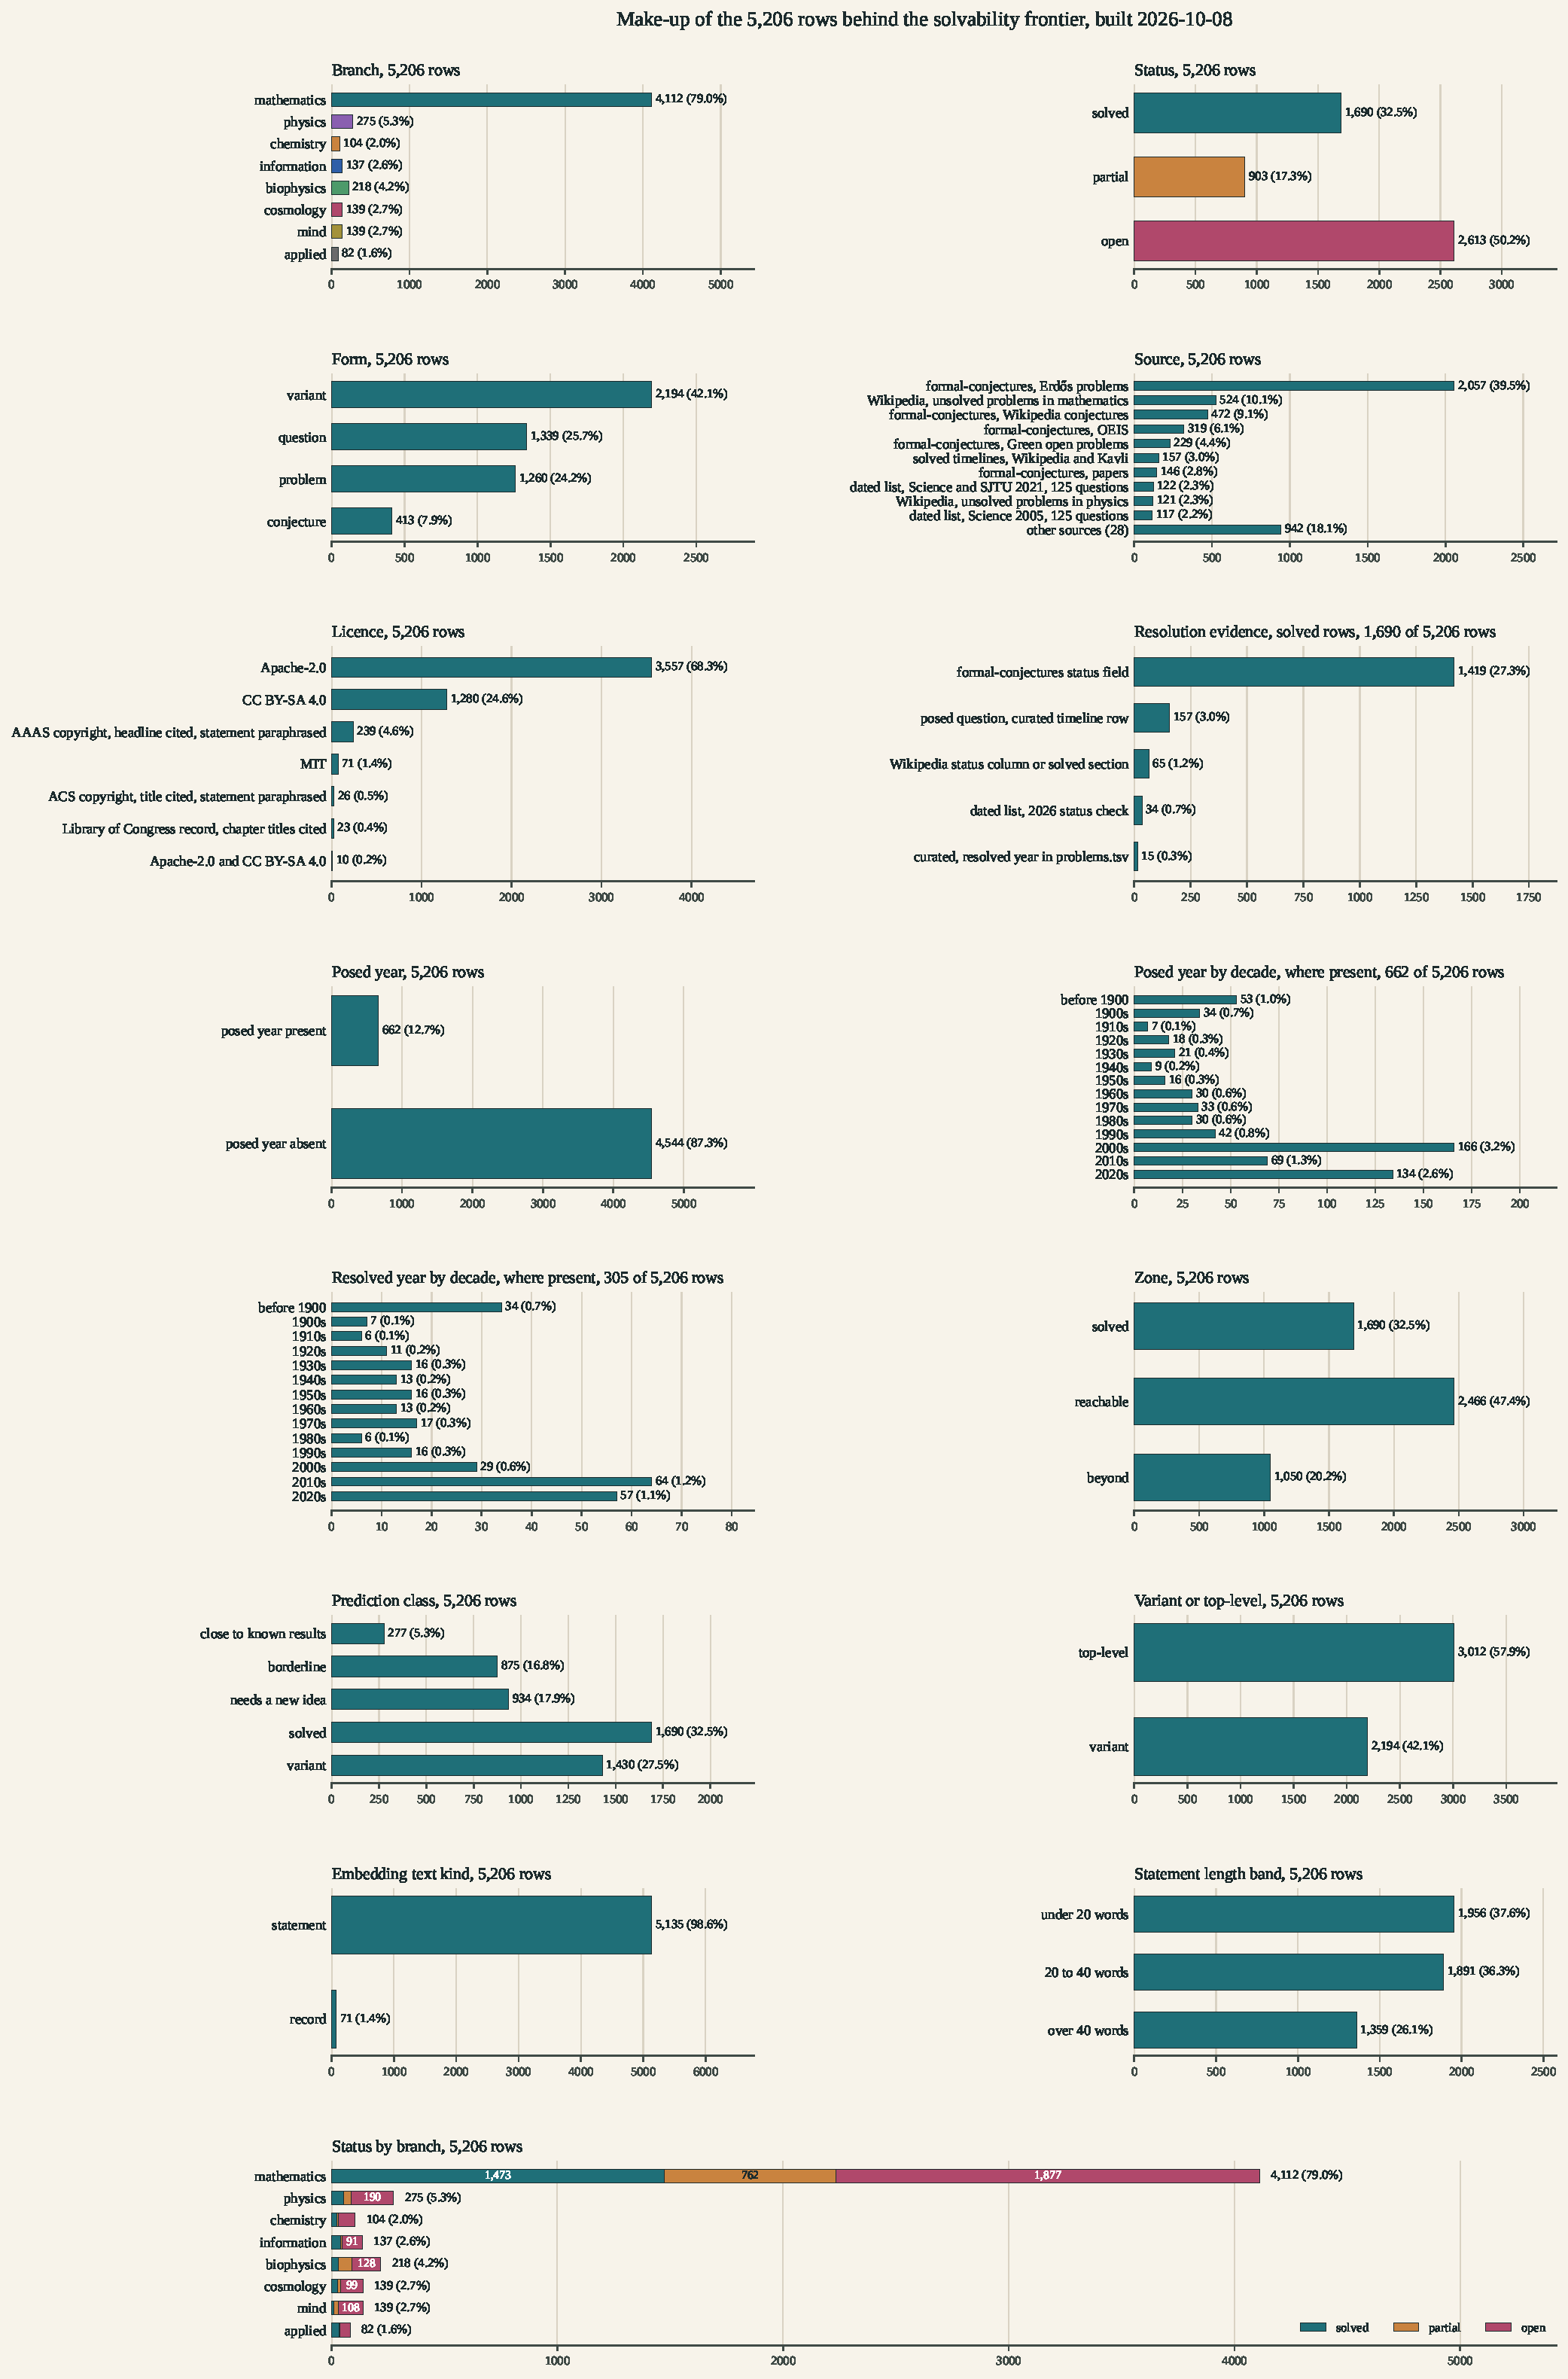
\includegraphics[width=\linewidth]{figures/fig_makeup.pdf}
  \caption{Make-up of the 5,080 rows by branch, status, form, source, licence, resolved kind, posed and resolved years, zone, prediction class, variant or top-level, embedding text kind and statement length, with status by branch \mk.}
  \label{fig:makeup}
\end{figure}

\subsection{Pipeline}

Each step names its formula; $i$ and $j$ index rows.

\begin{enumerate}
  \item \textbf{Text.} $t_i$ is the ingested statement when present, else the atlas problem record (name, aliases, statement, keywords, key work titles), else name plus keywords: 5,009 statement, 71 record and 0 name plus keywords rows \mk. The branch word never enters the text.
  \item \textbf{Embedding.} $e_i = f(t_i)/\lVert f(t_i)\rVert$ with $f$ = bge-small-en-v1.5 at revision 5c38ec7, 384 dimensions, cached by model revision and text hash \fr.
  \item \textbf{Similarity.} $s_{ij} = e_i \cdot e_j$, the cosine. The 50 highest $s_{ij}$ per row are stored to three decimals, with the nearest solved row over the whole set \fr.
  \item \textbf{Solved set.} $S = \{\, i : \mathrm{status}_i = \text{solved} \wedge (\mathrm{parent}_i = \varnothing \vee \mathrm{status}_{\mathrm{parent}_i} = \text{solved}) \,\}$, so a proved special case of an open problem stays partial; $|S| = 1{,}621$ \fr.
  \item \textbf{Reach.} $r_i = \max_{j \in S,\, j \neq i} s_{ij}$ over the stored neighbours and the stored nearest solved row (\Cref{def:reach}).
  \item \textbf{Threshold.} $\tau = Q_{0.1}(\{ r_j : j \in S \})$, the value at index $\lfloor 0.1\,|S| \rfloor$ of the sorted solved reaches; $\tau = 0.781$ \fr.
  \item \textbf{Zones.} solved if $i \in S$; unsampled if the branch holds fewer than 10 solved rows; reachable if $r_i \geq \tau$; beyond if $r_i < \tau$: 1,621, 103, 2,225 and 1,131 rows \fr.
  \item \textbf{Radius.} With $\mathrm{span}(x,a,b) = \min(1,\max(0,(x-a)/(b-a)))$: $\rho_i = 0.6\,(1 - \mathrm{span}(r_i, \min_S r, 1))$ for solved rows, $0.6 + 0.4\,(1 - \mathrm{span}(r_i, \tau, 1))$ for reachable rows, and $1 + 0.5\,(1 - \mathrm{span}(r_i, r_{\min}, \tau))$ beyond, where $r_{\min}$ is the smallest reach in the set \fr.
  \item \textbf{Growth.} $g_i = 1 + |\{\, j \in N_i : \mathrm{zone}_j = \text{beyond},\ j \text{ top-level},\ s_{ij} \geq \tau \,\}|$ over the 50 stored neighbours $N_i$ (\Cref{def:growth}).
  \item \textbf{Angle.} $p_i = (e_i - \bar e)\,V_2$ with $V_2$ the first two right singular vectors of the centred embeddings; $\theta_i$ is the rank of $\operatorname{atan2}(p_{i2}, p_{i1})$ over the rows, scaled to $[0, 2\pi)$ \fr.
  \item \textbf{Reach class.} $u = Q_{0.75}(\{ r_i : i \text{ open, inside} \}) = 0.854$ \pr; close when $r_i \geq u$, borderline when $\tau \leq r_i < u$, needs a new idea when $r_i < \tau$, unsampled by branch (\Cref{def:class}).
  \item \textbf{Backtest statistic.} At cutoff $c$: $d_c = p_{\mathrm{in}} - p_{\mathrm{out}}$ with $p$ the resolved share of scored rows on each side of $\tau_c$; ratio $p_{\mathrm{in}}/p_{\mathrm{out}}$, undefined when $p_{\mathrm{out}} = 0$ \bm{BucketMath.Marketing.ratio}; AUC $= \Pr(r_{\text{resolved}} > r_{\text{unresolved}})$ with ties at one half (\Cref{def:backtest}).
  \item \textbf{Permutation test.} $p = (1 + |\{ b : |d^*_b| \geq |d_c| \}|)/(B+1)$ with $B = 10{,}000$ shuffles of the outcomes across the inside and outside rows under seed 20261006 \bt, so $0 < p \leq 1$ (\Cref{app:lean}).
\end{enumerate}

\paragraph{OpenAlex activity.}
A title-and-abstract search on each sourced row's name or first clause, run against the OpenAlex works index with a key, stores the matching work count, counts per year for the last 30 years and the three most cited works per row in \texttt{tools/solvability-atlas/openalex-sourced.json}. The free daily budget is 1,000 requests, two per row, so 499 of the 5,009 rows are stored at this date, 388 of them with at least one matching work, median 15 works for mathematics \mk. The frontier score does not use these counts yet; \Cref{fig:makeup} carries no activity axis and the distribution by branch sits in the page's make-up charts.

\section{Results}
\label{sec:results}

\subsection{The frontier}

\begin{figure}[htbp]
  \centering
  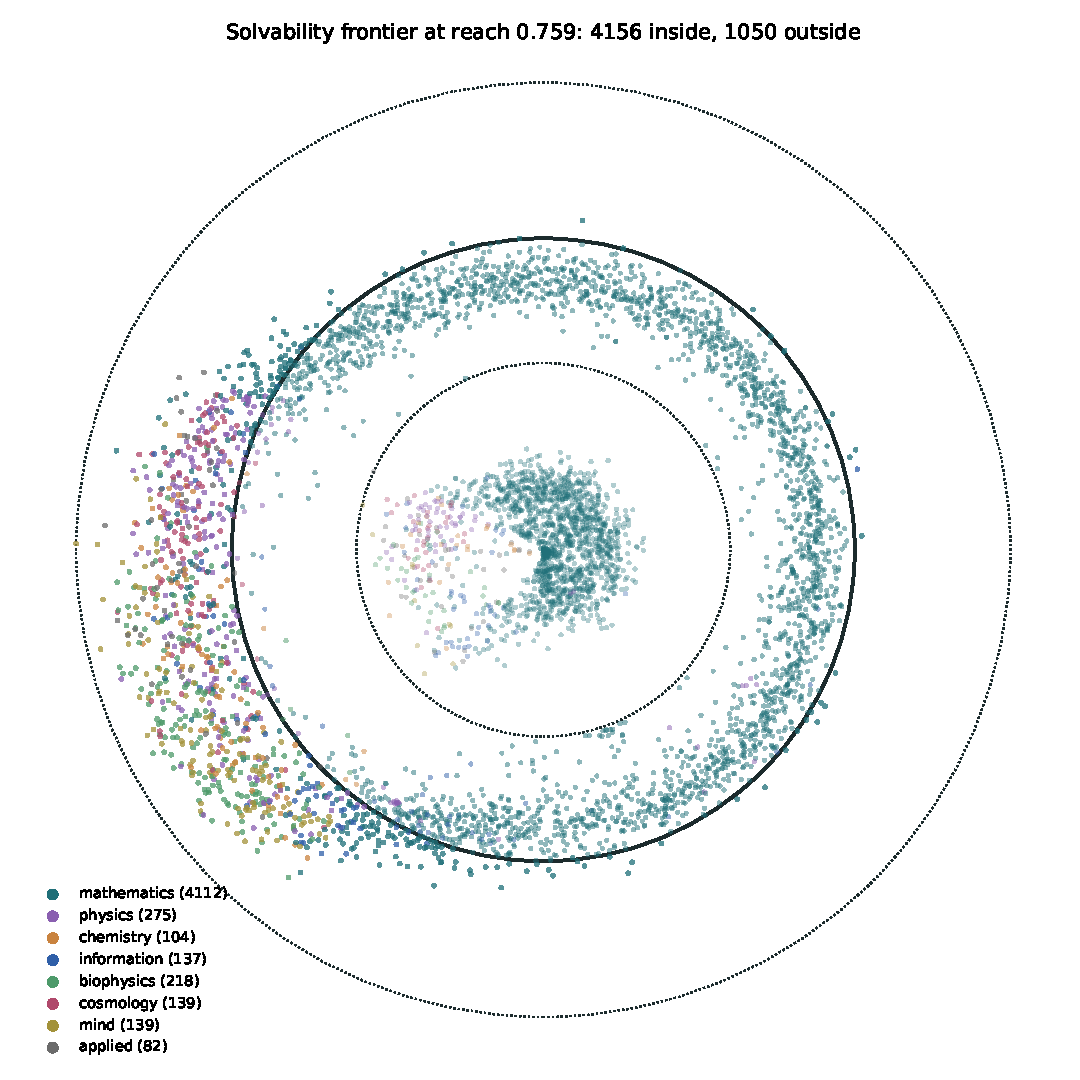
\includegraphics[width=0.9\linewidth]{figures/fig_frontier.pdf}
  \caption{The frontier on 5,080 rows. Solved rows fill the inner disc by reach, open rows inside fill the ring up to the circle at 0.781, outside rows sit beyond it by how far their reach falls short, and unsampled rows are grey crosses \fr. Angle is the row's rank along the first two principal components of the embeddings.}
  \label{fig:frontier}
\end{figure}

The frontier sits at $\tau = 0.781$: 1,621 rows solved, 2,225 reachable, 1,131 beyond and 103 unsampled, 3,846 inside and 1,234 outside \fr. \Cref{tab:branches} gives the split per branch. Mathematics holds 4,112 of the 5,080 rows and 1,473 of the 1,621 solved ones \fr, so it sets the threshold on its own.

\begin{table}[htbp]
  \centering
  \caption{Rows per branch and zone \fr.}
  \label{tab:branches}
  \small
  \begin{tabular}{@{}lrrrrrrr@{}}
\toprule
Branch & Total & Solved & Reachable & Beyond & Unsampled & Inside & Outside \\
\midrule
mathematics & 4112 & 1473 & 2171 & 468 & 0 & 3644 & 468 \\
physics & 259 & 37 & 28 & 194 & 0 & 65 & 194 \\
biophysics & 208 & 21 & 4 & 183 & 0 & 25 & 183 \\
cosmology & 127 & 16 & 0 & 111 & 0 & 16 & 111 \\
information & 115 & 29 & 19 & 67 & 0 & 48 & 67 \\
mind & 108 & 5 & 0 & 0 & 103 & 5 & 103 \\
chemistry & 85 & 13 & 3 & 69 & 0 & 16 & 69 \\
applied & 66 & 27 & 0 & 39 & 0 & 27 & 39 \\
\bottomrule
\end{tabular}

\end{table}

\subsection{Backtest}

\Cref{tab:bt2005s}, \Cref{tab:bt2005a}, \Cref{tab:bt2021s}, \Cref{tab:bt2021a} and \Cref{fig:backtest} hold the backtest. At cutoff 2005, 108 rows were solved by then, 16 of them with no solved neighbour among the 50 stored and dropped from the threshold, which came out at 0.644; 287 rows were posed by 2005 and open at the cutoff, 38 unsampled, 66 undecided and 183 scored \bt. At cutoff 2021, 190 rows were solved by then, 11 dropped, threshold 0.656; 465 rows tested, 58 unsampled, 43 undecided and 364 scored \bt.

\paragraph{Settled only.}
At 2005 the inside rows settle at 21\% over 112 against 6\% over 71 outside, ratio 3.804, $p=0.006$, AUC 0.800 \bt. At 2021 they settle at 12\% over 238 against 1\% over 126, ratio 14.824, $p=0.000$, AUC 0.883 \bt. The settled rows number 28 at 2005 and 29 at 2021 \bt. Of the tested rows, 32 at 2005 and 33 at 2021 are solved today with no resolved year, 11 and 21 of them scored; with those removed the inside rate falls to 13\% against 6\% (ratio 2.285, $p=0.131$, AUC 0.700) and to 3\% against 1\% (ratio 4.065, $p=0.269$, AUC 0.700) \bt. Most of the settled-only gap is those rows.

\paragraph{Settled or advanced.}
At 2005 the inside rate is 46\% against 61\% outside, ratio 0.752, $p=0.051$, AUC 0.479; at 2021 it is 43\% against 39\%, ratio 1.102, $p=0.503$, AUC 0.523 \bt. With the undated solved rows removed: 40\% against 61\% ($p=0.008$) and 37\% against 39\% ($p=0.818$) \bt.

\paragraph{Undecided rows.}
The 66 undecided rows at 2005 resolve at 32\% settled and 53\% settled or advanced; the 43 at 2021 at 28\% and 53\% \bt. Placing all of them inside or all outside gives, settled only, inside rates of 25\% or 21\% against 6\% or 18\% at 2005 and 14\% or 12\% against 1\% or 8\% at 2021; settled or advanced, 48\% or 46\% against 61\% or 57\% at 2005 and 45\% or 43\% against 39\% or 43\% at 2021 \bt. The last rows of each table carry the exact counts.

\begin{table}[htbp]
  \centering
  \caption{Backtest at cutoff 2005, settled only, by stratum; the last two rows place the undecided rows all inside and all outside \bt.}
  \label{tab:bt2005s}
  \small
  \begin{tabular}{@{}lrrrrrr@{}}
\toprule
Stratum & Inside & Outside & Resolved in & Resolved out & Ratio & $p$ \\
\midrule
all & 112 & 71 & 21\% & 6\% & 3.804 & 0.006 \\
all, undated solved rows removed & 101 & 71 & 13\% & 6\% & 2.285 & 0.131 \\
under 20 words & 28 & 20 & 7\% & 0\% &  & 0.503 \\
20 to 40 words & 44 & 36 & 14\% & 6\% & 2.455 & 0.282 \\
over 40 words & 40 & 15 & 40\% & 13\% & 3.000 & 0.102 \\
applied & 4 & 3 & \multicolumn{4}{l}{under 10 on one side} \\
biophysics & 18 & 44 & 11\% & 4\% & 2.444 & 0.577 \\
chemistry & 7 & 2 & \multicolumn{4}{l}{under 10 on one side} \\
cosmology & 11 & 5 & \multicolumn{4}{l}{under 10 on one side} \\
mathematics & 49 & 1 & \multicolumn{4}{l}{under 10 on one side} \\
physics & 23 & 16 & 30\% & 12\% & 2.435 & 0.263 \\
\midrule
all undecided inside & 178 & 71 & 25\% & 6\% & 4.487 & \\
all undecided outside & 112 & 137 & 21\% & 18\% & 1.174 & \\
\bottomrule
\end{tabular}

\end{table}

\begin{table}[htbp]
  \centering
  \caption{Backtest at cutoff 2005, settled or advanced, by stratum \bt.}
  \label{tab:bt2005a}
  \small
  \begin{tabular}{@{}lrrrrrr@{}}
\toprule
Stratum & Inside & Outside & Resolved in & Resolved out & Ratio & $p$ \\
\midrule
all & 159 & 67 & 47\% & 58\% & 0.810 & 0.148 \\
all, undated solved rows removed & 148 & 67 & 43\% & 58\% & 0.743 & 0.053 \\
under 20 words & 33 & 24 & 48\% & 62\% & 0.776 & 0.424 \\
20 to 40 words & 73 & 29 & 53\% & 76\% & 0.704 & 0.045 \\
over 40 words & 53 & 14 & 38\% & 14\% & 2.642 & 0.120 \\
applied & 8 & 3 & \multicolumn{4}{l}{under 10 on one side} \\
biophysics & 29 & 33 & 72\% & 76\% & 0.956 & 0.780 \\
chemistry & 7 & 2 & \multicolumn{4}{l}{under 10 on one side} \\
cosmology & 12 & 4 & \multicolumn{4}{l}{under 10 on one side} \\
information & 20 & 2 & \multicolumn{4}{l}{under 10 on one side} \\
mathematics & 50 & 0 & \multicolumn{4}{l}{under 10 on one side} \\
mind & 6 & 12 & \multicolumn{4}{l}{under 10 on one side} \\
physics & 27 & 11 & 41\% & 27\% & 1.494 & 0.485 \\
\midrule
all undecided inside & 231 & 67 & 48\% & 58\% & 0.833 & \\
all undecided outside & 159 & 139 & 47\% & 55\% & 0.863 & \\
\bottomrule
\end{tabular}

\end{table}

\begin{table}[htbp]
  \centering
  \caption{Backtest at cutoff 2021, settled only, by stratum \bt.}
  \label{tab:bt2021s}
  \small
  \begin{tabular}{@{}lrrrrrr@{}}
\toprule
Stratum & Inside & Outside & Resolved in & Resolved out & Ratio & $p$ \\
\midrule
all & 268 & 155 & 10\% & 1\% & 16.194 & $<$0.001 \\
all, undated solved rows removed & 247 & 155 & 3\% & 1\% & 4.393 & 0.151 \\
under 20 words & 119 & 76 & 1\% & 0\% &  & 1.000 \\
20 to 40 words & 91 & 52 & 7\% & 2\% & 3.429 & 0.264 \\
over 40 words & 58 & 27 & 36\% & 0\% &  & $<$0.001 \\
applied & 13 & 11 & 0\% & 0\% &  & 1.000 \\
biophysics & 43 & 48 & 2\% & 0\% &  & 0.471 \\
chemistry & 30 & 16 & 3\% & 0\% &  & 1.000 \\
cosmology & 19 & 11 & 0\% & 0\% &  & 1.000 \\
information & 23 & 7 & \multicolumn{4}{l}{under 10 on one side} \\
mathematics & 87 & 1 & \multicolumn{4}{l}{under 10 on one side} \\
mind & 24 & 34 & 0\% & 0\% &  & 1.000 \\
physics & 29 & 27 & 3\% & 0\% &  & 1.000 \\
\midrule
all undecided inside & 310 & 155 & 13\% & 1\% & 20.000 & \\
all undecided outside & 268 & 197 & 10\% & 7\% & 1.583 & \\
\bottomrule
\end{tabular}

\end{table}

\begin{table}[htbp]
  \centering
  \caption{Backtest at cutoff 2021, settled or advanced, by stratum \bt.}
  \label{tab:bt2021a}
  \small
  \begin{tabular}{@{}lrrrrrr@{}}
\toprule
Stratum & Inside & Outside & Resolved in & Resolved out & Ratio & $p$ \\
\midrule
all & 272 & 167 & 43\% & 40\% & 1.063 & 0.615 \\
all, undated solved rows removed & 251 & 167 & 38\% & 40\% & 0.943 & 0.677 \\
under 20 words & 122 & 81 & 38\% & 41\% & 0.946 & 0.773 \\
20 to 40 words & 92 & 59 & 46\% & 58\% & 0.792 & 0.183 \\
over 40 words & 58 & 27 & 47\% & 0\% &  & $<$0.001 \\
applied & 15 & 13 & 13\% & 15\% & 0.867 & 1.000 \\
biophysics & 41 & 50 & 66\% & 66\% & 0.998 & 1.000 \\
chemistry & 27 & 19 & 18\% & 21\% & 0.880 & 1.000 \\
cosmology & 19 & 11 & 47\% & 27\% & 1.737 & 0.442 \\
information & 23 & 8 & \multicolumn{4}{l}{under 10 on one side} \\
mathematics & 96 & 2 & \multicolumn{4}{l}{under 10 on one side} \\
mind & 24 & 34 & 25\% & 44\% & 0.567 & 0.169 \\
physics & 27 & 30 & 26\% & 27\% & 0.972 & 1.000 \\
\midrule
all undecided inside & 315 & 167 & 44\% & 40\% & 1.108 & \\
all undecided outside & 272 & 210 & 43\% & 43\% & 0.984 & \\
\bottomrule
\end{tabular}

\end{table}

\begin{figure}[htbp]
  \centering
  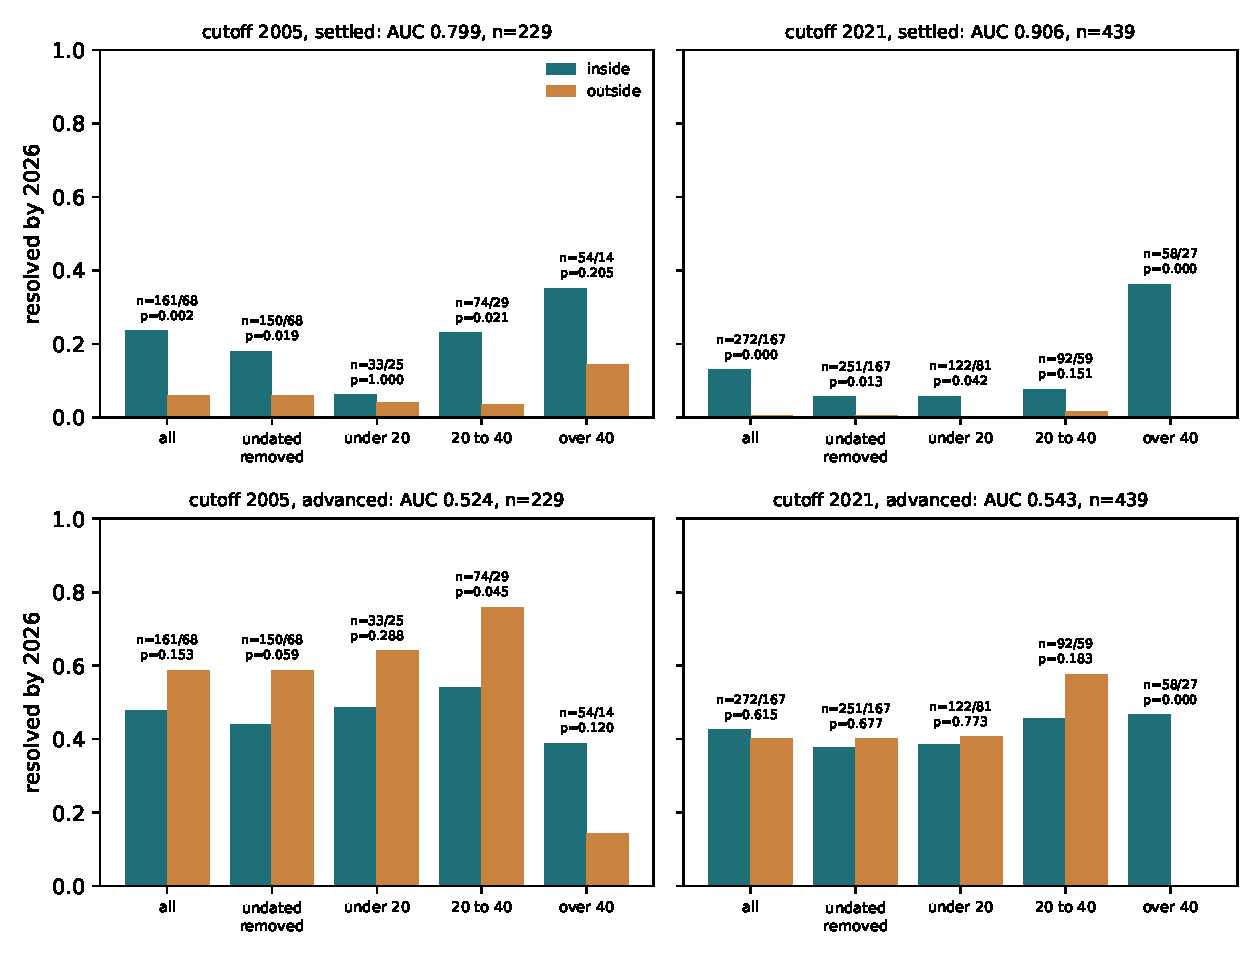
\includegraphics[width=\linewidth]{figures/fig_backtest.pdf}
  \caption{Resolved rate by 2026 inside and outside the cutoff frontier under both codings, over all scored rows, with the undated solved rows removed, and by length band \bt.}
  \label{fig:backtest}
\end{figure}

Under settled or advanced, two strata reach $p$ below 0.05 and run against each other: at 2005 the 20 to 40 word band resolves at 46\% inside against 75\% outside ($p=0.013$), while at 2021 the over 40 word band resolves at 45\% inside against 0\% outside over 20 rows ($p=0.000$) \bt. The second is a cohort effect: the long statements outside at 2021 are the 2021 list's own longer paraphrases, all still open five years on \bt. Mathematics scores one row outside at both cutoffs \bt, because nearly every dated mathematics row has a solved mathematics neighbour, so no mathematics rate is given.

\subsection{Where this is weak}
\label{sec:weak}

\paragraph{Partial.}
The two codings disagree on sign at 2005 and on size at 2021. Partial was assigned in 2026 by the ingest from a status page, with no threshold for how much progress counts, so the column that decides the result is the least reliable one in the file.

\paragraph{Leakage.}
The embeddings and the 50 stored neighbours come from the 2026 corpus. Statements written after a cutoff, including the 2021 list when scoring 2005, shape the geometry each cutoff is scored on, and the nearest solved row at a cutoff was found among neighbours chosen in 2026. The test checks the rule against known outcomes under that leak, which is a weaker claim than a forecast. A clean version needs embeddings fitted on text dated at or before the cutoff and a neighbour set frozen per cutoff.

\paragraph{Vocabulary.}
Cosine similarity between statement embeddings measures shared words and phrasing. Two problems can share a method and no vocabulary, or vocabulary and no method.

\paragraph{Mathematics.}
4,112 of 5,080 rows and 1,473 of 1,621 solved rows are mathematics \fr. The threshold is a mathematics quantity, and the other six branches are read against it.

\paragraph{Two cohorts.}
Of the 517 rows with a posed year, 241 come from the 2005 and 2021 Science lists, and those two lists supply most of the tested rows at both cutoffs \bt. A list's paraphrases share length and style, which is what the length bands are for, and the over 40 word result at 2021 shows the cohort rather than the rule \bt.

\paragraph{The 50-neighbour bound.}
At a cutoff with few solved rows, most of a row's solved peers fall outside its 50 stored neighbours, so its reach is unknown: 66 rows undecided and 16 solved rows dropped at 2005, 43 and 11 at 2021 \bt. Dropping them can only raise the threshold; the undecided bounds above show how far they can move the inside rate.

\paragraph{Resolved years.}
Only 224 of the 1,621 solved rows carry a resolved year, so the solved set at a cutoff, 108 at 2005 and 190 at 2021, is a fraction of what was solved by then \bt, and 32 and 33 solved rows with no year sit in the tested set instead.

\subsection{Predictions}

\Cref{tab:counts} gives the class counts: 251 rows close to known results, 764 borderline, 911 that need a new idea and 103 unsampled, with $u = 0.854$ \pr. \Cref{tab:top0}, \Cref{tab:top1}, \Cref{tab:top2} and \Cref{tab:top3} list the first ten of each class by growth; the full ranked table with the three nearest solved problems and the starting works is \texttt{predictions.csv}. \Cref{app:atlas} lists the 56 open atlas problems in full. Among them, Goldbach and the Langlands program are close to known results, with reach 0.867 and 0.863 to an Erdős problem and to the geometric Langlands conjecture \pr; the Riemann hypothesis, Navier-Stokes, dark matter, weak cosmic censorship and quantum gravity head the \enquote{needs a new idea} class by growth, 4, 4, 3, 3 and 3 \pr. The Goldbach placement is the vocabulary effect of \Cref{sec:weak}: the nearest solved row shares the words, and nothing in the method says whether it shares a method.

\begin{table}[htbp]
  \centering
  \caption{Open top-level problems per reach class \pr.}
  \label{tab:counts}
  \begin{tabular}{@{}lr@{}}
\toprule
Class & Open problems \\
\midrule
close to known results & 268 \\
borderline & 863 \\
needs a new idea & 954 \\
unsampled & 0 \\
\bottomrule
\end{tabular}

\end{table}

\begin{figure}[htbp]
  \centering
  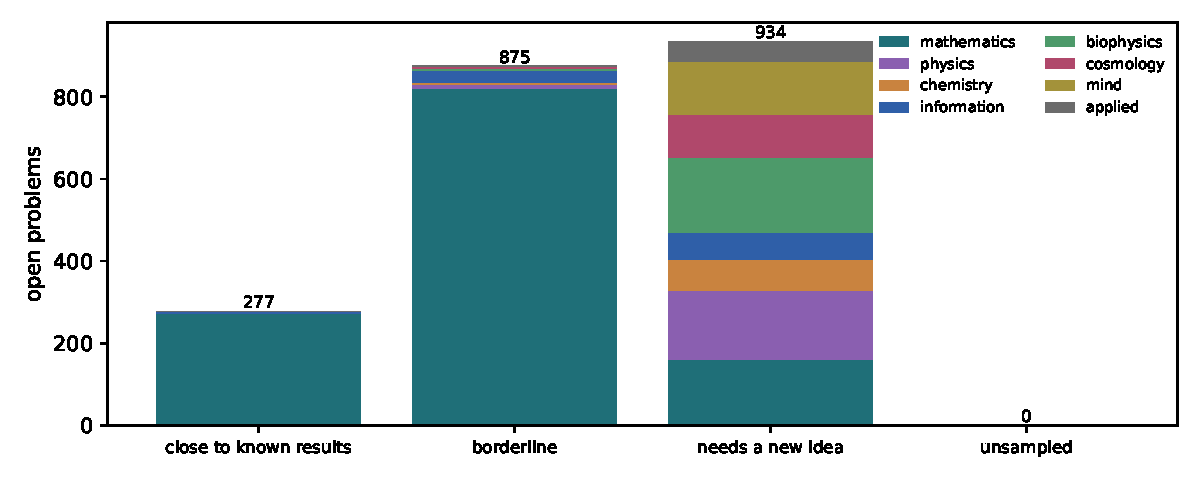
\includegraphics[width=\linewidth]{figures/fig_classes.pdf}
  \caption{Reach classes by branch \pr.}
  \label{fig:classes}
\end{figure}

\begin{table}[htbp]
  \centering
  \caption{Close to known results, first ten by growth \pr.}
  \label{tab:top0}
  \footnotesize
  \begin{tabular}{@{}p{0.42\linewidth}lrrp{0.3\linewidth}@{}}
\toprule
Problem & Branch & Reach & Growth & Nearest solved \\
\midrule
Pierpont Prime, infinitely many pierpont primes & mathematics & 0.870 & 4 & Regular Primes, infinitude of irregularprimes \\
Can the graph isomorphism problem be solved in polynomial time on a classical computer? & information & 0.924 & 3 & Graph isomorphism in quasi-polynomial time \\
Wieferich Prime, infinite isWieferichPrime & mathematics & 0.871 & 3 & Regular Primes, infinitude of irregularprimes \\
OEIS A945, every prime occurs & mathematics & 0.868 & 2 & OEIS A363102, a eq one or prime \\
Factorial Prime, infinitely many factorial primes & mathematics & 0.908 & 1 & Regular Primes, infinitude of irregularprimes \\
Caratheodory conjecture & mathematics & 0.894 & 1 & Caratheodory conjecture for surfaces of smoothness C\^{}\{4\} (Brendan Guil \\
Is graph canonization polynomial-time equivalent to the graph isomorphism problem? & information & 0.887 & 1 & Graph isomorphism in quasi-polynomial time \\
Erdos problem 1030 & mathematics & 0.882 & 1 & Erdos problem 1014 \\
Erdos problem 968 & mathematics & 0.882 & 1 & Erdos problem 822 \\
OEIS A93818 & mathematics & 0.878 & 1 & OEIS A372761, exists unique a eq prime \\
\bottomrule
\end{tabular}

\end{table}

\begin{table}[htbp]
  \centering
  \caption{Borderline, first ten by growth \pr.}
  \label{tab:top1}
  \footnotesize
  \begin{tabular}{@{}p{0.42\linewidth}lrrp{0.3\linewidth}@{}}
\toprule
Problem & Branch & Reach & Growth & Nearest solved \\
\midrule
Cerny conjecture & information & 0.776 & 4 & Undirected connectivity in logarithmic space \\
Can all-pairs shortest paths be computed in strongly sub-cubic time, that is, in time for  & information & 0.766 & 4 & Lovasz Plummer Conjecture, explicit \\
The Kobon triangle problem on triangles in line arrangements & mathematics & 0.805 & 3 & Erdos problem 619, h three le \\
Lebesgue's universal covering problem on the minimum-area convex shape in the plane that c & mathematics & 0.789 & 3 & Talagrand's convexity conjecture (Dongming Hua, Antoine Song, Stefan T \\
Are the nim-sequences of all finite octal games eventually periodic? & mathematics & 0.788 & 3 & Erdos problem 198, concrete \\
Finite lattice representation problem & mathematics & 0.782 & 3 & Modularity Conjecture \\
Banach Mazur Rotation & mathematics & 0.772 & 3 & Mazur's conjecture B (Vessilin Dimitrov, Ziyang Gao, and Philipp Habeg \\
Proton decay and spin crisis & physics & 0.766 & 3 & Internal structure of the proton \\
Dubner's conjecture & mathematics & 0.841 & 2 & Erdos problem 418, conditional \\
The Hadwiger?Nelson problem on the chromatic number of unit distance graphs & mathematics & 0.833 & 2 & Disproof of Hedetniemi's conjecture on the chromatic number of tensor  \\
\bottomrule
\end{tabular}

\end{table}

\begin{table}[htbp]
  \centering
  \caption{Needs a new idea, first ten by growth \pr.}
  \label{tab:top2}
  \footnotesize
  \begin{tabular}{@{}p{0.42\linewidth}lrrp{0.3\linewidth}@{}}
\toprule
Problem & Branch & Reach & Growth & Nearest solved \\
\midrule
Dynamical neuroscience & mind & 0.706 & 14 & Experience-driven reorganisation of the brain \\
Computational neuroscience & biophysics & 0.702 & 14 & Undirected connectivity in logarithmic space \\
Can we understand the action of brain in natural environments? & mind & 0.695 & 14 & Chemical neurotransmission at synapses \\
Cosmological principle & physics & 0.721 & 13 & Baryon acoustic oscillations \\
Connectionism & mind & 0.706 & 12 & Undirected connectivity in logarithmic space \\
Free will, particularly the neuroscience of free will & mind & 0.696 & 11 & Keller's conjecture (Joshua Brakensiek, Marijn Heule, John Mackey, Dav \\
To what extent is the brain reconfigurable? & mind & 0.686 & 11 & Experience-driven reorganisation of the brain \\
Computational theory of mind & biophysics & 0.677 & 10 & Erdos problem 152 \\
Consciousness & biophysics & 0.661 & 9 & Chemical neurotransmission at synapses \\
Cognition and decisions & biophysics & 0.660 & 9 & Experience-driven reorganisation of the brain \\
\bottomrule
\end{tabular}

\end{table}

\begin{table}[htbp]
  \centering
  \caption{Unsampled, first ten by growth \pr.}
  \label{tab:top3}
  \footnotesize
  \begin{tabular}{@{}p{0.42\linewidth}lrrp{0.3\linewidth}@{}}
\toprule
Problem & Branch & Reach & Growth & Nearest solved \\
\midrule
\bottomrule
\end{tabular}

\end{table}

\section{Calibration}
\label{sec:calibration}

The central claims are empirical, so the calibration is the backtest itself: the rule is fixed before the outcomes are read, the outcomes are the 2026 status column with its per-row source, and the threshold and the strata are recomputed at each cutoff from rows dated at or before it. The error budget is the permutation $p$-value, the stratum floor, the two codings and the two bounded exclusions. Under settled only the inside rows settle at a higher rate at both cutoffs, and most of that gap is the solved rows with no resolved year; under settled or advanced the AUC sits at 0.479 and 0.523, each within 0.03 of chance \bt. The reading is that the result turns on the partial column, and no forecast claim survives the embedding leak of \Cref{sec:weak}.

\section{Limitations}
\label{sec:limitations}

\Cref{sec:weak} lists the weak points of the backtest and the frontier: the partial column, the 2026 embedding leak, vocabulary as similarity, mathematics dominance, the two cohorts, the 50-neighbour bound and the missing resolved years.

\paragraph{Sources and licences.}
\texttt{problems.tsv} is MIT. formal-conjectures rows are Apache-2.0. Wikipedia lists and the DARPA and XPRIZE rows are CC BY-SA 4.0 with attribution in the data. The Science 2005 and 2021 lists, the systems-neuroscience chapter titles and the Holy Grails titles are cited as headlines under 15 words with paraphrased statements, since the bodies are under copyright. The encoder is MIT.

\printbibliography

\appendix

\section{Glossary}
\label{app:glossary}

\printglossaryentry{reach}
\printglossaryentry{frontier}
\printglossaryentry{growth}
\printglossaryentry{reachclass}
\printglossaryentry{backtest}

\section{The atlas problems}
\label{app:atlas}

\footnotesize
\begin{longtable}{@{}p{0.3\linewidth}llrrp{0.3\linewidth}@{}}
\toprule Problem & Class & Branch & Reach & Growth & Nearest solved \\ \midrule \endhead
\bottomrule \endfoot
Goldbach conjecture & reach & mathematics & 0.867 & 0 & Erdos problem 418, conditional \\
Langlands program & reach & mathematics & 0.863 & 0 & Geometric Langlands conjecture \\
Graph isomorphism complexity & borderline & information & 0.833 & 0 & Graph isomorphism in quasi-polynomial time \\
Jacobian conjecture & borderline & mathematics & 0.807 & 0 & Poisson Conjecture, jacobian implication \\
Collatz conjecture & borderline & mathematics & 0.786 & 0 & OEIS A306424, forty three is max \\
Riemann hypothesis & needs a new idea & mathematics & 0.771 & 4 & Deterministic polynomial-time primality testing \\
Navier-Stokes existence and smoothness & needs a new idea & physics & 0.671 & 4 & Poincare, smooth known cases \\
Dark matter identity & needs a new idea & cosmology & 0.678 & 3 & Baryon acoustic oscillations \\
Weak cosmic censorship & needs a new idea & cosmology & 0.659 & 3 & Baryon acoustic oscillations \\
Quantum gravity & needs a new idea & cosmology & 0.615 & 3 & Microscopic Weighting, iff finite concentration \\
Room-temperature superconductivity mechanism & needs a new idea & physics & 0.603 & 3 & Element predicted as eka-aluminium \\
Programmed versus stochastic aging & needs a new idea & biophysics & 0.602 & 3 & Carrier of hereditary information \\
Glass transition & needs a new idea & chemistry & 0.601 & 3 & Continuum hypothesis independence \\
Integer factoring complexity & needs a new idea & information & 0.752 & 2 & OEIS A382590, kthPrimeFactor periodic \\
Hadwiger-Nelson problem & needs a new idea & mathematics & 0.743 & 2 & Erdos problem 780 \\
Invariant subspace problem & needs a new idea & mathematics & 0.727 & 2 & Green open problem 49 \\
Matrix multiplication exponent omega & needs a new idea & information & 0.725 & 2 & OEIS A108306 \\
Existence of one-way functions & needs a new idea & information & 0.711 & 2 & Erdos problem 198, concrete \\
Hubble tension & needs a new idea & cosmology & 0.707 & 2 & Expansion of the universe \\
BQP vs BPP separation & needs a new idea & information & 0.693 & 2 & Graph isomorphism in quasi-polynomial time \\
Yang-Mills mass gap & needs a new idea & physics & 0.693 & 2 & Microscopic Weighting, iff finite concentration \\
Black hole information paradox & needs a new idea & cosmology & 0.691 & 2 & Ultraviolet catastrophe \\
Origin of life & needs a new idea & biophysics & 0.688 & 2 & Urea synthesis from inorganic reagents \\
Cosmological constant problem & needs a new idea & cosmology & 0.668 & 2 & Erdos problem 1005, constant \\
Quantum measurement problem & needs a new idea & physics & 0.637 & 2 & Einstein problem (David Smith, Joseph Samuel Myers, Craig S \\
Birch and Swinnerton-Dyer conjecture & needs a new idea & mathematics & 0.764 & 1 & Elliptic Curve Rank, goldfeld two le \\
abc conjecture & needs a new idea & mathematics & 0.760 & 1 & Erdos problem 494, k eq 3 card gt 6 \\
Unique Games Conjecture & needs a new idea & information & 0.751 & 1 & Complexity of computing Nash equilibria \\
Twin prime conjecture & needs a new idea & mathematics & 0.745 & 1 & OEIS A91669, prime and primitive root of dvd \\
P vs NP & needs a new idea & information & 0.732 & 1 & Complexity of computing Nash equilibria \\
Protein folding pathway kinetics & needs a new idea & biophysics & 0.721 & 1 & Protein structure prediction \\
Hodge conjecture & needs a new idea & mathematics & 0.714 & 1 & Poincare conjecture \\
Hadamard matrix conjecture & needs a new idea & mathematics & 0.706 & 1 & Gerstenhaber Three Matrices, exists finrank adjoin quadruple \\
Succinct proofs without trusted setup optimality & needs a new idea & information & 0.702 & 1 & Erdos problem 967, tauberian \\
Elliptic curve discrete log hardness & needs a new idea & information & 0.697 & 1 & Modularity Conjecture \\
Exact exchange-correlation functional & needs a new idea & chemistry & 0.683 & 1 & Erdos problem 298, natural density \\
Bioelectric pattern control & needs a new idea & biophysics & 0.681 & 1 & Chemical neurotransmission at synapses \\
Market efficiency as computational hardness & needs a new idea & information & 0.674 & 1 & Erdos problem 298, natural density \\
Fermion sign problem & needs a new idea & physics & 0.666 & 1 & Monochromatic Quantum Graph, eqSystem6 no solution d5 \\
Anomalous properties of water & needs a new idea & chemistry & 0.659 & 1 & Proof of the atomic theory \\
Climate sensitivity bound & needs a new idea & physics & 0.653 & 1 & Sensitivity conjecture \\
Autoformalization of mathematics & needs a new idea & information & 0.649 & 1 & 21 149, kourovka 21 149 not inner \\
Optimal multi-item auction design & needs a new idea & information & 0.649 & 1 & Complexity of computing Nash equilibria \\
2D Hubbard model ground state & needs a new idea & physics & 0.640 & 1 & Existence of time crystals (2012?2016) \\
Formal reasoning limits of transformers & needs a new idea & information & 0.637 & 1 & Erdos problem 152 \\
Mitochondrial redox and aging mechanism & needs a new idea & biophysics & 0.634 & 1 & Carrier of hereditary information \\
AI alignment verification & needs a new idea & information & 0.624 & 1 & Pandemic Response XPRIZE \\
Rough volatility pricing & needs a new idea & mathematics & 0.622 & 1 & Pricing of options \\
Turbulence closure & needs a new idea & physics & 0.617 & 1 & Voronovskaja Type Formula, bezier bernstein operators \\
Rational catalyst design & needs a new idea & chemistry & 0.598 & 1 & Complexity of computing Nash equilibria \\
Plasma confinement stability & needs a new idea & physics & 0.588 & 1 & Solar abundance problem (1998?2022) \\
Light, circadian biology and metabolism & needs a new idea & biophysics & 0.572 & 1 & OEIS A100478 \\
Smale's 18th problem limits of intelligence & unsampled & mind & 0.673 & 0 & Hilbert's tenth problem \\
Neural binding problem & unsampled & mind & 0.660 & 0 & Controlling neurons with light \\
Free energy principle formalization & unsampled & mind & 0.659 & 0 & Erdos problem 298, natural density \\
Hard problem of consciousness & unsampled & mind & 0.641 & 0 & Keller's conjecture (Joshua Brakensiek, Marijn Heule, John M \\
\end{longtable}

\normalsize

\section{Lean listings}
\label{app:lean}

\texttt{lean/Bucket/Backtest.lean}, checked by \texttt{make lean}, holds the two facts the method leans on: the corrected permutation $p$ has a positive numerator no larger than its denominator, and the length bands cover every word count.

\begin{lstlisting}[style=bucketlean]
structure PermutationP where
  hits : Nat
  permutations : Nat
  bounded : hits <= permutations

def PermutationP.numerator (p : PermutationP) : Nat := p.hits + 1
def PermutationP.denominator (p : PermutationP) : Nat := p.permutations + 1

theorem PermutationP.numerator_pos (p : PermutationP) : 0 < p.numerator :=
  Nat.succ_pos p.hits

theorem PermutationP.numerator_le_denominator (p : PermutationP) :
    p.numerator <= p.denominator :=
  Nat.succ_le_succ p.bounded

def lengthBand (words : Nat) : LengthBand :=
  if words < 20 then .short else if words <= 40 then .middle else .long

theorem lengthBand_total (words : Nat) :
    lengthBand words = .short \/ lengthBand words = .middle \/ lengthBand words = .long
\end{lstlisting}

\texttt{lake build} output, quoted verbatim \emp{papers/solvability-frontier/lean, 2026-10-06, make lean}.
% voice-ignore-next 3
\begin{verbatim}
Build completed successfully (4 jobs).
\end{verbatim}

\end{document}
